\documentclass[aspectratio=169]{beamer}
\usetheme{Pittsburgh}
\usecolortheme{spruce}
\usefonttheme{structurebold}
\beamertemplatenavigationsymbolsempty
\usepackage{graphicx}
\usepackage{tikz}
\usepackage{biber}

\title{Far Flung Forest Landscapes in the Anthropocene}
\subtitle{Structural analysis of China's embodied forest network}
\author{M.K. Lau (Ph.D.)}
\institute{Chinese Academy of Sciences and Harvard University}


\begin{document}

\begin{frame}
  \titlepage
\end{frame}

\section*{Context}

\begin{frame}
  \frametitle{Forests are Important}

  \begin{itemize}
  \item Carbon Storage
  \item Water and nutrient cycling
  \item resources(wood, food)
  \item Biodiversity
  \item Human Health and Culture
  \end{itemize}

\end{frame}


\begin{frame}
  \frametitle{Forests in the Anthropocence}
  
  \begin{itemize}
  \item Forests are changing from human impacts
  \item Large effects of land-use
  \item How do we assess direct and indirect effects?
  \item How do we address systems-level effects?
  \end{itemize}

\end{frame}


\begin{frame}
  \frametitle{Today's Talk}

\tableofcontents

%% - Intro/Context
%%   - Forests are globally important
%%   - Anthropocence effects 
%%   - Global forest loss and gain and change
%% 	- Global greening = India(Agriculture) + China(Forests)
%% - Economics*Ecology = Landscape Extended Models
%% - Network Analysis of China's Greening
%%   - Global Scale
%%   - Local Scale
%% 	- Landscape = Chen 2019
%% 	- Resilience Analysis of China's Forest LE-MRIO
%% - Conclusions and Future Work
%% - Acknowledgements

\end{frame}



\section{Economic and Ecological Landscape Extensions}

  %% - Global forest loss and gain and change
  %% - Global greening = India(Agriculture) + China(Forests)


\section{Trade Networks of Forest Landscapes}

\section{Global Forest Networks}


\section{China's Forest Networks: Global}


\section{China's Forest Networks: Domestic/Local}

%%   - Local Scale
%% 	- Landscape = Chen 2019
%% 	- Resilience Analysis of China's Forest LE-MRIO

\section{Conclusions}

\section{Future Work}

\begin{frame}
  \frametitle{Acknowledgements}
\end{frame}



{ % all template changes are local to this group.
    \setbeamertemplate{navigation symbols}{}
    \begin{frame}<article:0>[plain]
      \frametitle{Q \& A}
        \begin{tikzpicture}[remember picture,overlay]
            \node[at=(current page.center)] {
                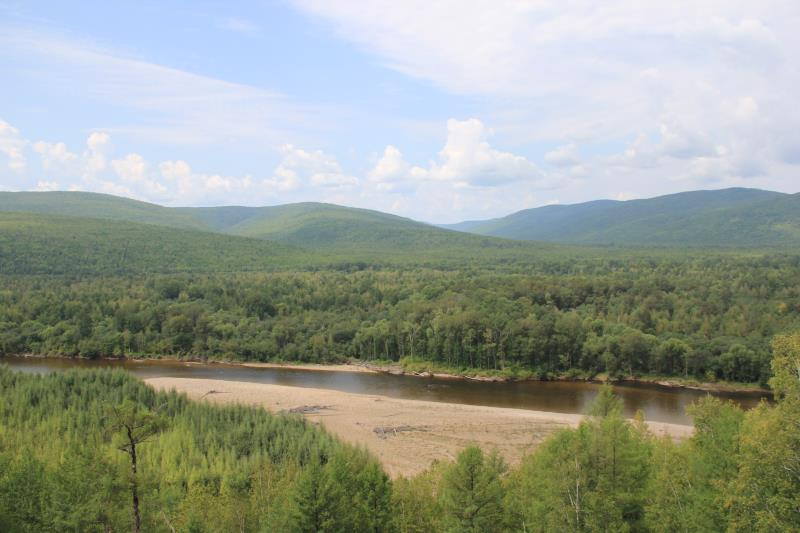
\includegraphics[keepaspectratio,
                                 width=\paperwidth]{images/CNF/IMG_0199.JPG}
            };
        \end{tikzpicture}
     \end{frame}
}

\begin{frame}
  \parencite{Burgess2012}    
  \cite{Caggiani2014}
  \cite{Carvalho2019AdaptationSystems}
  \cite{Schaffer-Smith2018NetworkTrade}
\end{frame}


\begin{frame}[allowframebreaks]
  \frametitle{References}
  \tiny \bibliography{biblio.bib}
  \bibliographystyle{abbrv}
\end{frame}


\end{document}
